\section{General}
	\subsection{Terms and Definitions}
		\begin{table}[H]
			\centering
			\begin{tabular}{|>{\bfseries}p{0.2\linewidth}|p{0.75\linewidth}|}
				 \hline
				 CPU bound
				 	& Algorithms that use bursts of CPU time.\\
				 \hline
				 I/O bound  
				 	& Algorithms that spend much time waiting for I/O\\
				 \hline		
				 Row major order  
				 	& In multidimensional arrays row elements are stored next to each other (C/C++, Pascal\ldots)\\
				 \hline
				 Column major order  
				 	& In multidimensional arrays column elements are stored next to each other (Matlab, \ldots)\\
				\hline
			\end{tabular}
		\end{table}
	
	\subsection{Elements of an FPGA \weekMaehne{1}}
		\begin{longtable}{|p{0.475\textwidth}|p{0.475\textwidth}|}
			\hline
			\textbf{Look-Up-Table (LUT:)}
			
			Any logic function can be expressed as a sum of products.
				
				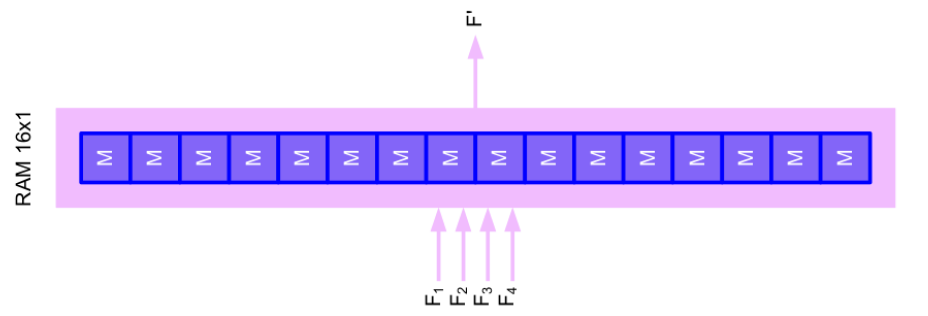
\includegraphics[width=0.4\textwidth]{./pictures/LUT.png}
				& \textbf{Basic Logic Element (BLE) or Logic Cell:}
				
					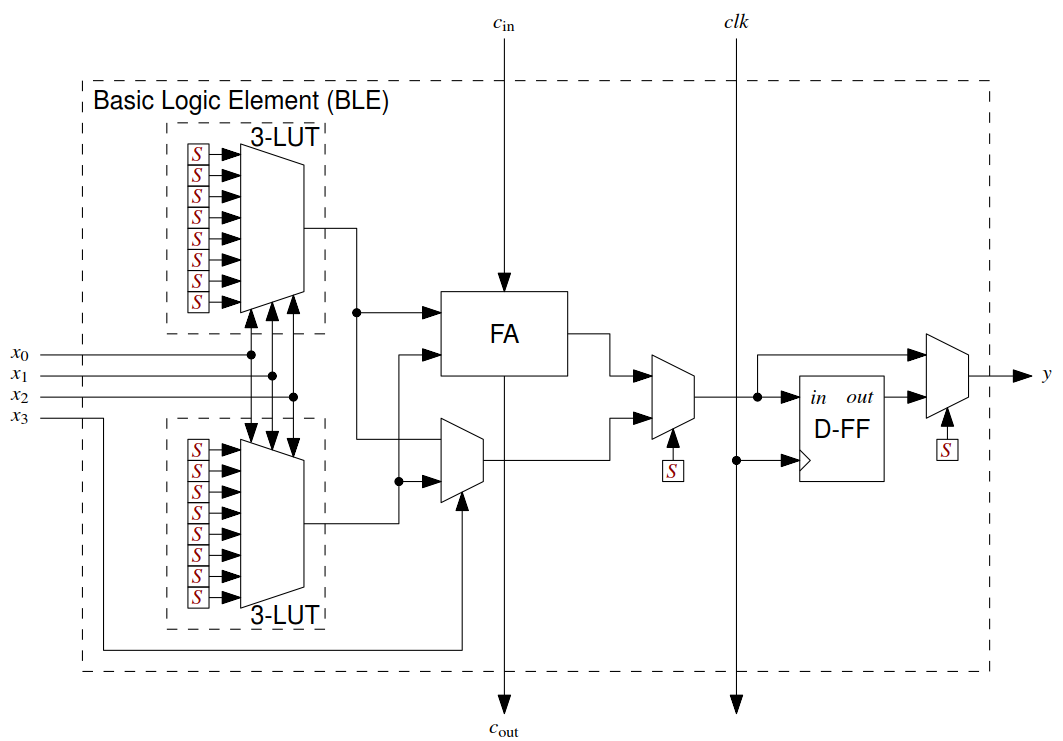
\includegraphics[width=0.4\textwidth]{./pictures/ble.png}\\
			\hline
			\textbf{Switch Box (SB), Connection Box (CB):}
			
				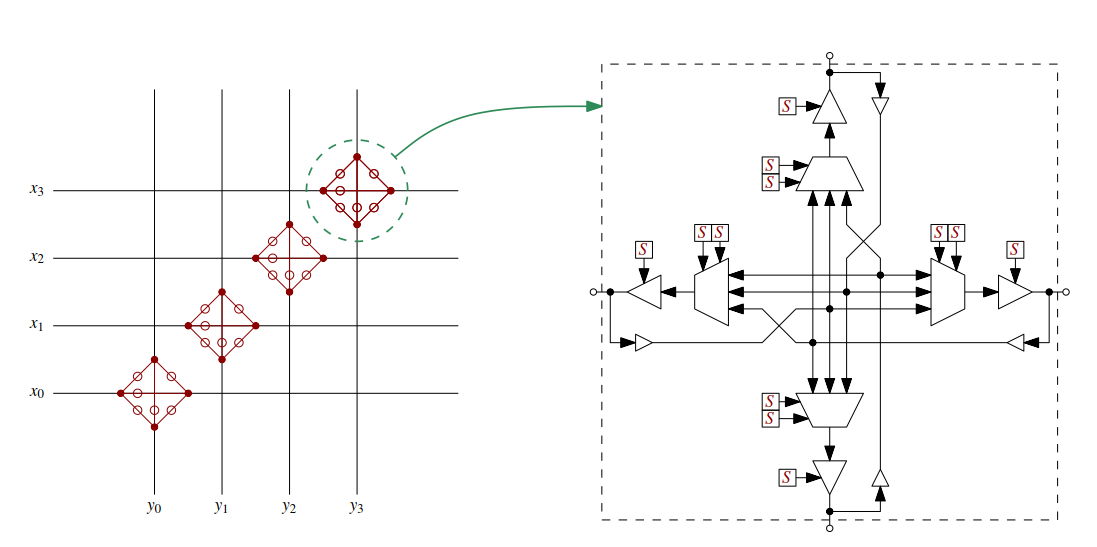
\includegraphics[width=0.4\textwidth]{./pictures/sb.png}
				& \textbf{Configurable Logic Block (CLB):}
				
				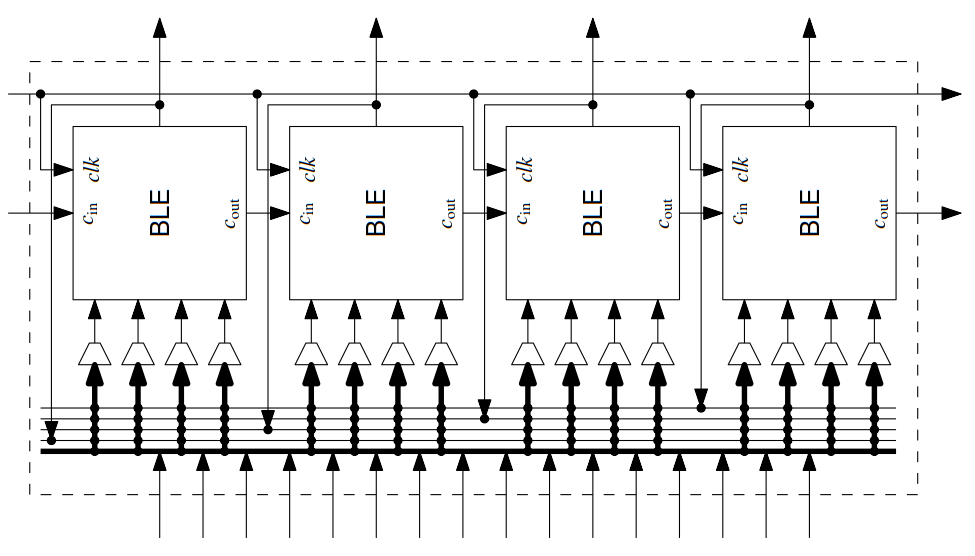
\includegraphics[width=0.4\textwidth]{./pictures/clb.png} \\
			\hline		
			\textbf{Input/Output block (IOB):}
			
				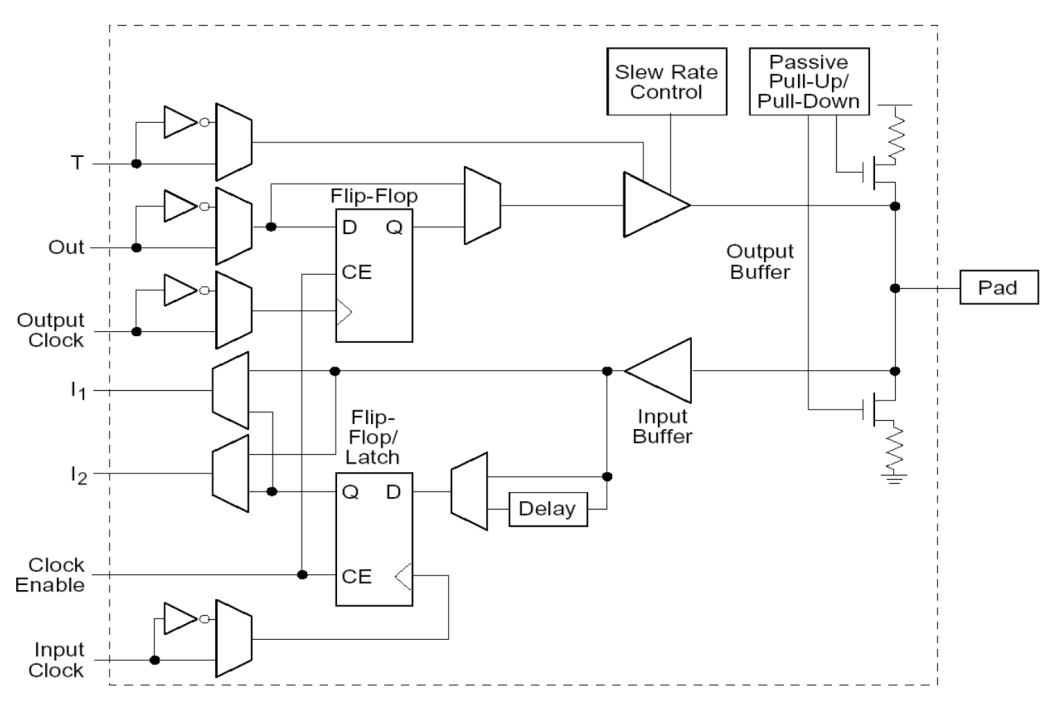
\includegraphics[width=0.4\textwidth]{./pictures/iob.png}
				& \textbf{Dedicated Blocks (DBs):}
				
				Configurable specialized blocks
				implementing commonly needed functionality efficiently
				\begin{compactitem}
					\item Block SRAM
					\item Digital Clock Manager (DCM), DLL, PLL
					\item Multiplier
					\item DSP block
					\item Complete CPU cores
				\end{compactitem}\\
			\hline
		\end{longtable}
		
	